\documentclass[a4paper,fleqn]{article}

%\usepackage{times}

\usepackage[margin = 2.5 cm]{geometry}
\usepackage[utf8]{inputenc}
\usepackage[T1]{fontenc}
\usepackage{tabularx}
\usepackage{graphicx}
\usepackage{subfigure}
\usepackage{tikz}
\usetikzlibrary{trees}
\usepackage{hyperref}
\usepackage{amsmath}
\usepackage{xcolor}
\usepackage{gensymb}
\usepackage{amsfonts}
\usepackage{natbib}
\usepackage{float} 
\usepackage[font=it]{caption}

\bibliographystyle{abbrv}
\usetikzlibrary{positioning,shadows}

\begin{document}

\title{Percolation model\\ \Large{Report}}
\author{Tim Schön}
\date{}
\maketitle
\ \\

\section*{Percolation model}
In 1957 Broadbent and Hammersley researched the flow of substances through porous media. They introduced a theory today called \emph{bond percolation} to model this process. \cite{PercWW}\\
For this, they simplified the porous medium as a graph, namely a grid, with edges, modeling the pores. For this purpose, the edges can be activated to allow flow through them, or deactivated. The porosity of the medium influences a probability $p$, which is the probability that an edge is active. \cite{Percolation}\\
This leads to some questions one can study:
\begin{enumerate}
	\item What is the size of the largest connected component of the graph, $S_G(p)$, only using active edges? 
	\item How is this size dependent on the propability $p$ and the type of graph $G$?
	\item At which probability does a so called \emph{percolation event} likely occur, that is, the size of the connected component neares the size of the graph?
	\item When does a path from the top to the bottom, using only active edges, exist?
\end{enumerate}
I tried to answer some of these questions using an implementation in python, visualized with \emph{PyQt}.
\section*{Implementation using \emph{Python} with \emph{PyQt}}
In this demo application different grids and gridsizes can be chosen with a graphical 
user interface. The graph will then be visualized using OpenGL, after randomly drawing active edges using the value $p$, which can be varied by the user.
Additionally, the application will find the connected components of the graph and calculate the fraction $\frac{S(p)}{|V|}$ for the largest connected component found. Breadth-first-search (BFS) is used to find the connected components for the subgraph of active edges.\\
To further visualize the percolation effect, a shortest path from the top to the bottom of the graph is found and visualized, if it exists. For this, the A* algorithm is used.\\
The value of $p$ and the corresponding $S(p)$ found by this analysis is added to a scatterplot of observations, which will be grown slowly as the user changes any of the input values.
\begin{figure}[H]
	\includegraphics*[width=\textwidth]{images/screen1}
	\caption{The demo application, showing percolation through an $99 \times 99$ triangular, two-dimensional grid. The blue path shows a path from the top to the bottom.}	\label{screenshot}
\end{figure}
\subsection*{Installing and running the application}
This application relies on \verb|PyQT5| for the graphical user interface, \verb|PyOpenGL| for the drawing of the graph and \verb|pyqtgraph| for rendering the scatterplot. Additionally, \verb|numpy| is used for some calculations under the hood.\\
Nevertheless, installing these dependencies should, thanks to \verb|pip|, be as simple as running
\begin{center}
	\verb|pip3 install -r requirements.txt|
\end{center}
from the root folder of the application. If everything was successful, you can then run the application using Python 3: \verb|python3 main.py|.
\subsection*{Usage and GUI}
Figure \ref{screenshot} shows the graphical user interface of the application.\\
On the left side the user controls and the scatterplot is located. The following parameters can be controlled by the user:
\begin{itemize}
	\item Type of the grid used. For the moment, only \emph{2D-(rectangular)-grid}, \emph{2D-triangles}, \emph{2D-honycomb} and \emph{3D-grid} can be chosen as grid types. This can be extended in the future thanks to the implementation of the grid types.
	\item The parameter $p$ controlling the propability that an edge is active. If this parameter is changed, the state of each edge is drawn from an bernoulli distribution with probability $p$.
	\item The grid size $N$. If this parameter is changed, the grid is reconstructed and refreshed.
	\item Wether all edges should be redrawn from the distribution when $p$ is changed. If this is not checked, the application will keep count of the active edges. If the number of active edges divided by the number of all edges is less than $p$, it will select edges to activate randomly, until ist is equal to $p$; if the number of active edges divided by all edges is more than $p$, it will select edges randomly and deactivate them accordingly. \\
	This doesn't really change anything in regards to the observed percolation thresholds, but it does look cool.
\end{itemize}
Below the user controls the scatter plot is rendered. Everytime the grid is \emph{refreshed}, i.e. the state of the edges is redrawn, a point is added to it, indicating $p$ and the maximum observed cluster size. It can be cleared by the user with the button below it.\\
The left side of the application consists of the graph drawing widget, rendering the graph and showing statistics. Shown is the current value of $p$, the number of nodes, active edges and all edges.
\subsection*{Implemented grid types and results}
The different grid types were programmed as different classes, each inheriting a common class (\verb|Graph|), which supports different essential algorithms for finding the connected 
components and shortest paths. Initially, the graphs are generated as a list of nodes as an numpy array with spatial coordinates and a list of edges, each storing the indices of the connected nodes.
To execute the A* and breadth-first-search algorithms the graph is transformed in adjacency-list-format beforehand.
\subsubsection*{Square 2D-grid}
\begin{figure}[H]
	\centering
	\begin{minipage}{0.4\textwidth}
		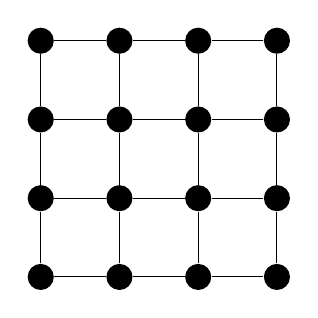
\begin{tikzpicture}
			\node[circle, fill=black] (11) at (0,0) {};
			\node[circle, fill=black] (12) at (0,1) {};
			\node[circle, fill=black] (13) at (0,2) {};
			\node[circle, fill=black] (14) at (0,3) {};
			\node[circle, fill=black] (21) at (1,0) {};
			\node[circle, fill=black] (22) at (1,1) {};
			\node[circle, fill=black] (23) at (1,2) {};
			\node[circle, fill=black] (24) at (1,3) {};
			\node[circle, fill=black] (31) at (2,0) {};
			\node[circle, fill=black] (32) at (2,1) {};
			\node[circle, fill=black] (33) at (2,2) {};
			\node[circle, fill=black] (34) at (2,3) {};
			\node[circle, fill=black] (41) at (3,0) {};
			\node[circle, fill=black] (42) at (3,1) {};
			\node[circle, fill=black] (43) at (3,2) {};
			\node[circle, fill=black] (44) at (3,3) {};
			
			\draw (11) -- (21) -- (31) -- (41);
			\draw (12) -- (22) -- (32) -- (42);
			\draw (13) -- (23) -- (33) -- (43);
			\draw (14) -- (24)-- (34) -- (44);
			\draw (11) -- (12) -- (13) -- (14);
			\draw (21) -- (22) -- (23) -- (24);
			\draw (31) -- (32) -- (33) -- (34);
			\draw (41) -- (42) -- (43) -- (44);
		\end{tikzpicture}
	\end{minipage}
	\begin{minipage}{0.3\textwidth}
	
	\includegraphics*[width=\textwidth]{images/2dgrid}
	\end{minipage}
\caption{$S(p)-p$-graph for the percolation of a $99\times 99$ sqaure grid. Percolation seems to occur at around $p \approx 0.5$, consistent with the theoretical results of \cite{Percolation}, $\frac{1}{2} = 0.5$ }
\end{figure}
\subsubsection*{Triangle 2D-grid}
\begin{figure}[H]
	\centering
	\begin{minipage}{0.4\textwidth}
		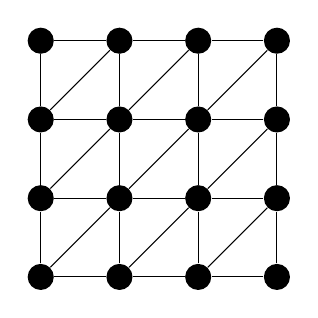
\begin{tikzpicture}
		\node[circle, fill=black] (11) at (0,0) {};
		\node[circle, fill=black] (12) at (0,1) {};
		\node[circle, fill=black] (13) at (0,2) {};
		\node[circle, fill=black] (14) at (0,3) {};
		\node[circle, fill=black] (21) at (1,0) {};
		\node[circle, fill=black] (22) at (1,1) {};
		\node[circle, fill=black] (23) at (1,2) {};
		\node[circle, fill=black] (24) at (1,3) {};
		\node[circle, fill=black] (31) at (2,0) {};
		\node[circle, fill=black] (32) at (2,1) {};
		\node[circle, fill=black] (33) at (2,2) {};
		\node[circle, fill=black] (34) at (2,3) {};
		\node[circle, fill=black] (41) at (3,0) {};
		\node[circle, fill=black] (42) at (3,1) {};
		\node[circle, fill=black] (43) at (3,2) {};
		\node[circle, fill=black] (44) at (3,3) {};
		
		\draw (11) -- (21) -- (31) -- (41);
		\draw (12) -- (22) -- (32) -- (42);
		\draw (13) -- (23) -- (33) -- (43);
		\draw (14) -- (24)-- (34) -- (44);
		\draw (11) -- (12) -- (13) -- (14);
		\draw (21) -- (22) -- (23) -- (24);
		\draw (31) -- (32) -- (33) -- (34);
		\draw (41) -- (42) -- (43) -- (44);
		\draw (11) -- (22) -- (33) -- (44);
		\draw (12) -- (23)-- (34);
		\draw (13) -- (24);
		\draw (21) -- (32) -- (43);
		\draw (31) -- (42);
		\end{tikzpicture}
	\end{minipage}
\begin{minipage}{0.3\textwidth}
\includegraphics*[width=\textwidth]{images/2dtriangles}
\end{minipage}
\caption{$S(p)-p$-graph for the percolation of a $99\times 99$ triangular grid. Percolation seems to occur at around $p \approx 0.35$, consistent with the theoretical results of \cite{Percolation}, $2\sin(\frac{\pi}{18}) \approx 0.34729$ }
\end{figure}
\subsubsection*{Honeycomb 2D-grid}
\begin{figure}[H]
	\centering
	\begin{minipage}{0.3\textwidth}
		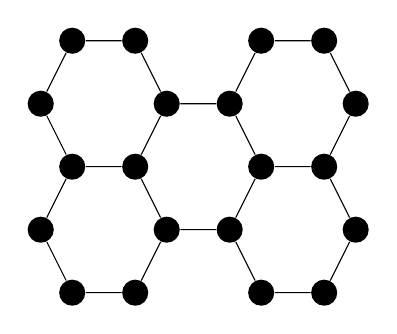
\begin{tikzpicture}[scale=0.8]
		\node[circle, fill=black] (11) at (0.5,0) {};
		\node[circle, fill=black] (12) at (0,1) {};
		\node[circle, fill=black] (13) at (0.5,2) {};
		\node[circle, fill=black] (14) at (0,3) {};
		\node[circle, fill=black] (15) at (0.5,4) {};
		\node[circle, fill=black] (21) at (1.5,0) {};
		\node[circle, fill=black] (23) at (1.5,2) {};
		\node[circle, fill=black] (25) at (1.5,4) {};
		\node[circle, fill=black] (32) at (2,1) {};
		\node[circle, fill=black] (34) at (2,3) {};
		\node[circle, fill=black] (42) at (3,1) {};
		\node[circle, fill=black] (44) at (3,3) {};
		
		\node[circle, fill=black] (51) at (3.5,0) {};
		\node[circle, fill=black] (53) at (3.5,2) {};
		\node[circle, fill=black] (55) at (3.5,4) {};
		\node[circle, fill=black] (61) at (4.5,0) {};
		\node[circle, fill=black] (63) at (4.5,2) {};
		\node[circle, fill=black] (65) at (4.5,4) {};		
		
		\node[circle, fill=black] (72) at (5,1) {};
		\node[circle, fill=black] (74) at (5,3) {};
		
		\draw (11) -- (12) -- (13) -- (23) -- (32) -- (21) -- (11);
		\draw (13) -- (14) -- (15) -- (25) -- (34) -- (23);
		\draw (34) -- (44) -- (53) -- (42) -- (32);
		\draw (53) -- (63) -- (72) -- (61) -- (51) -- (42);
		\draw (44) -- (55) -- (65) -- (74) -- (63);
		\end{tikzpicture}
	\end{minipage}
	\begin{minipage}{0.3\textwidth}		
		\includegraphics*[width=\textwidth]{images/2dhoneycomb}
	\end{minipage}
	\caption{$S(p)-p$-graph for the percolation of a $99\times 99$ honeycomb grid. Percolation seems to occur at around $p \approx 0.65$, consistent with the theoretical results of \cite{Percolation}, $1-2\sin(\frac{\pi}{18}) \approx 0.65271$ }
\end{figure}
\subsubsection*{Cubic 3D-grid}
\begin{figure}[H]
	\centering
	\begin{minipage}{0.3\textwidth}
		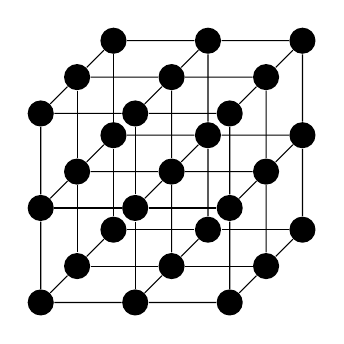
\begin{tikzpicture}[scale=1.2]
			\node[circle, fill=black](000) at (0,0,0) {};
			\node[circle, fill=black](001) at (0,0,1) {};
			\node[circle, fill=black](002) at (0,0,2) {};
			\node[circle, fill=black](010) at (0,1,0) {};
			\node[circle, fill=black](011) at (0,1,1) {};
			\node[circle, fill=black](012) at (0,1,2) {};
			\node[circle, fill=black](020) at (0,2,0) {};
			\node[circle, fill=black](021) at (0,2,1) {};
			\node[circle, fill=black](022) at (0,2,2) {};
			\node[circle, fill=black](100) at (1,0,0) {};
			\node[circle, fill=black](101) at (1,0,1) {};
			\node[circle, fill=black](102) at (1,0,2) {};
			\node[circle, fill=black](110) at (1,1,0) {};
			\node[circle, fill=black](111) at (1,1,1) {};
			\node[circle, fill=black](112) at (1,1,2) {};
			\node[circle, fill=black](120) at (1,2,0) {};
			\node[circle, fill=black](121) at (1,2,1) {};
			\node[circle, fill=black](122) at (1,2,2) {};
			\node[circle, fill=black](200) at (2,0,0) {};
			\node[circle, fill=black](201) at (2,0,1) {};
			\node[circle, fill=black](202) at (2,0,2) {};
			\node[circle, fill=black](210) at (2,1,0) {};
			\node[circle, fill=black](211) at (2,1,1) {};
			\node[circle, fill=black](212) at (2,1,2) {};
			\node[circle, fill=black](220) at (2,2,0) {};
			\node[circle, fill=black](221) at (2,2,1) {};
			\node[circle, fill=black](222) at (2,2,2) {};
			
			\draw (000) -- (001) -- (002);
			\draw (010) -- (011) -- (012);
			\draw (020) -- (021) -- (022);
			\draw (100) -- (101) -- (102);
			\draw (110) -- (111) -- (112);
			\draw (120) -- (121) -- (122);
			\draw (200) -- (201) -- (202);
			\draw (210) -- (211) -- (212);
			\draw (220) -- (221) -- (222);
			
			\draw (000) -- (010) -- (020);
			\draw (001) -- (011) -- (021);
			\draw (002) -- (012) -- (022);
			\draw (100) -- (110) -- (120);
			\draw (101) -- (111) -- (121);
			\draw (102) -- (112) -- (122);
			\draw (200) -- (210) -- (220);
			\draw (201) -- (211) -- (221);
			\draw (202) -- (212) -- (222);
			
			\draw (000) -- (100) -- (200);
			\draw (001) -- (101) -- (201);
			\draw (002) -- (102) -- (202);
			\draw (010) -- (110) -- (210);
			\draw (011) -- (111) -- (211);
			\draw (012) -- (112) -- (212);
			\draw (020) -- (120) -- (220);
			\draw (021) -- (121) -- (221);
			\draw (022) -- (122) -- (222);
		\end{tikzpicture}
	\end{minipage}	
	\begin{minipage}{0.3\textwidth}
		
		\includegraphics*[width=\textwidth]{images/3dgrid}
	\end{minipage}
\caption{$S(p)-p$-graph for the percolation of a $17 \times 17$ honeycomb grid. Percolation seems to occur at around $p \approx 0.27$, approximately consistent with the theoretical results of \cite{Percolation}, $0.2488$ }
\end{figure}
\bibliography{literature}

\end{document}